% Made up for the tikra benchmark.
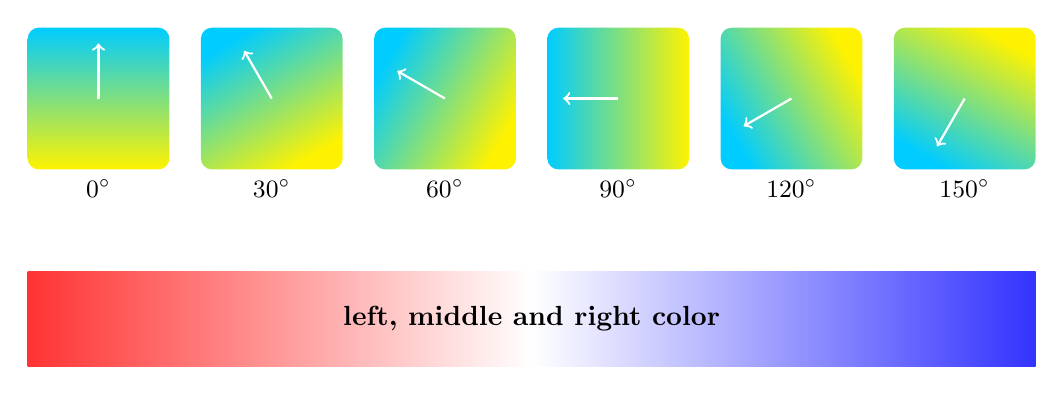
\begin{tikzpicture}
  \foreach \a [count=\i from 0] in {0,30,60,90,120,150} {
    \shade[top color=cyan!80!blue, bottom color=yellow!90!orange, shading angle=\a, rounded corners=4pt]
      (\i*2.2,0) rectangle +(1.8,1.8);
    \draw[->, thick, white] (\i*2.2+0.9,0.9) -- +(\a+90:0.7);
    \node[below, font=\small] at (\i*2.2+0.9,0) {\a$^\circ$};
  }
  \shade[left color=red!80, right color=blue!80, middle color=white] (0,-2.5) rectangle (12.8,-1.3);
  \node[font=\bfseries] at (6.4,-1.9) {left, middle and right color};
\end{tikzpicture}
